%pdflatex-../thesis.tex
% vim:spell spelllang=en_us

There are three models defining measurement tasks and result. Definition, session and transfer. There models are used to describe migration tasks instructions, migration progress and results. 



\subsection{Definition}
Definition model, formally MeasureDefinition, is used to save prescription for measurement task. It is possible to crate definition in console or using web interface. Screenshot can be seen in figure \ref{img:web-new-definition}.

Model have these parameters:
\begin{description}
	\item[vm] is virtual machine which is going to be migrated, list of \Ac{VM}s available for migration is loaded on-demand from orchestrator using OneOrchestrator class. Virtual machine must be in running state and variable \Code{THEMIS\_TYPE = 'VM'} need to be present in contextualization settings.
	\item[source] is source host for virtual machine. \Ac{VM} need to be migrated to this host before starting measurement session. List of hosts is loaded using OneOrchestrator class and hosts status is checked for every hosts.
	\item[destination] is destination host. \Ac{VM} is migrated to this host during measurement session.
	\item[bandwidth] 
	\item[cycles]
	\item[supervisor]
	\item[description]

	\item[started\_at]
	\item[finished\_at]
\end{description}

% connection with orchestrator


\begin{figure}[htb]
	\begin{center}
	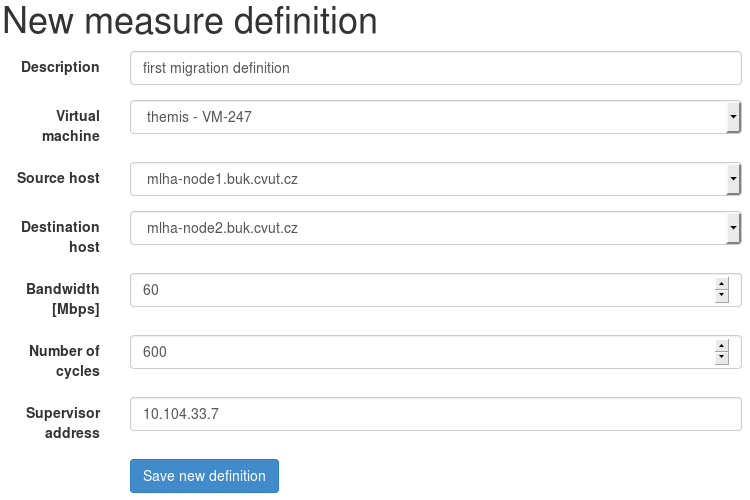
\includegraphics[width=0.9\textwidth]{form_measure_definition_new.png}
	\end{center}
	\caption{Web interface - new definition}
	\label{img:web-new-definition}
\end{figure}

	
\subsection{Session}

\subsection{Transfer}

% delayed job
